\documentclass{article}

\usepackage[brazil]{babel}
\usepackage{graphicx}
\usepackage{hyperref}
\usepackage{geometry}
\geometry{a4paper, margin=2cm}
\usepackage{siunitx}
\usepackage{subcaption}
\usepackage{hyperref}
\usepackage{float}

\setlength{\parindent}{0pt}
\setlength{\parskip}{0.5em}

\title{Acústica da Marimba}
\author{Gabriel Haruo Hanai Takeuchi (NUSP: 13671636)}
\date{}

\begin{document}

\maketitle

\section{Introdução}

A marimba é um instrumento de \textbf{percussão} da classe dos \textbf{idiofones} de \textbf{uma dimensão}. É composta por \textbf{barras}, que podem ser percutidas por \textbf{baquetas}, e \textbf{ressoadores}, que potencializam a intensidade do som.

\begin{figure}[h!]
  \centering
  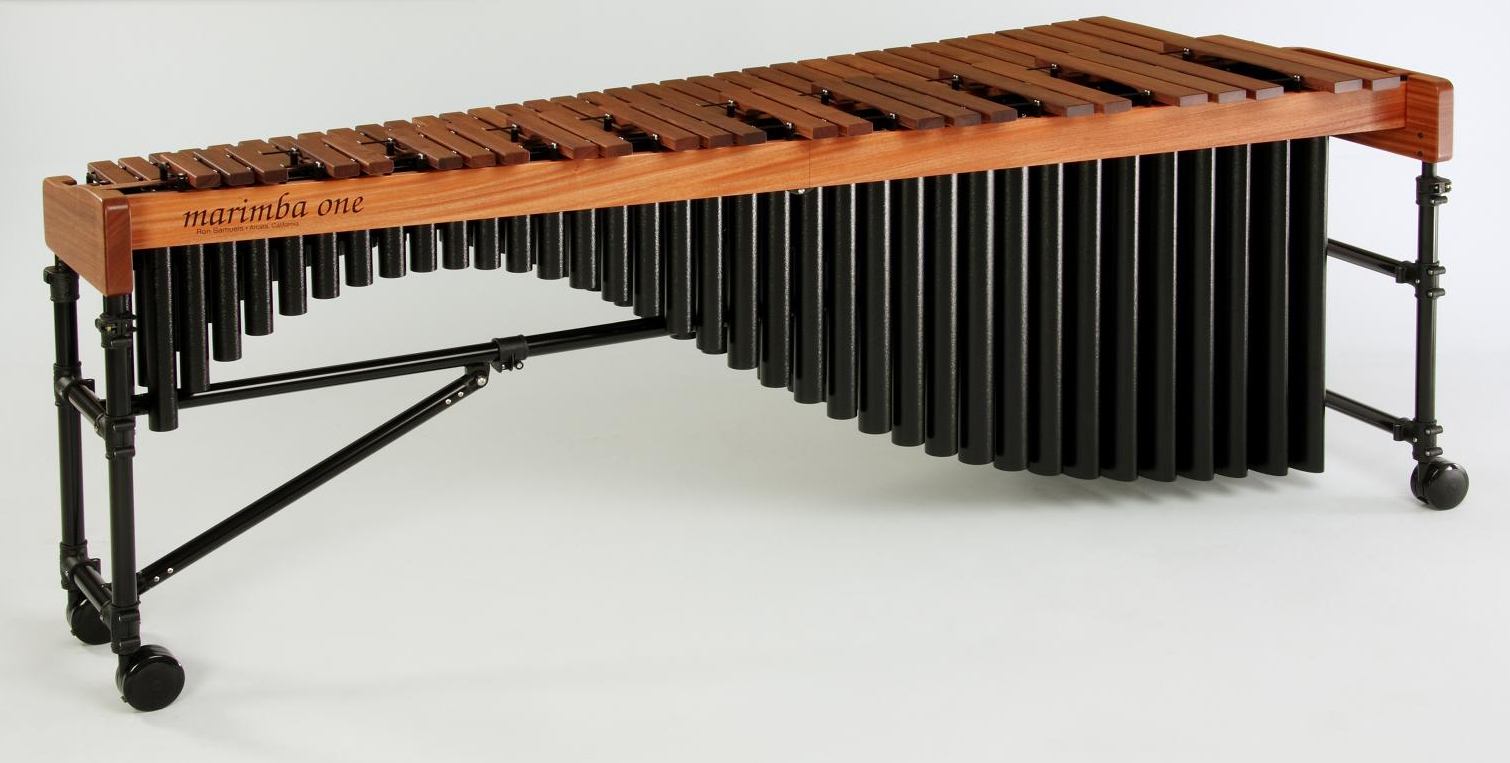
\includegraphics[width=0.8\textwidth]{Marimba_One_4000_Series.jpg}
  \caption{Marimba One 4000 Series~\cite{wiki:marimba}}
  \noindent 
\end{figure}

\section{Estrutura}

\subsection{Barras}

As barras (ou lâminas) da marimba são feitas de madeira de pau-rosa ou fibra de vidro. A espessura de uma barra é composta por extremidades mais grossas e uma região central mais fina (um arco escavado), o que permite uma afinação precisa ao controlar massa do objeto. A forma da barra é mostrada na imagem~\ref{fig:marimba_bars}.

\begin{figure}[h!]
	\centering
	\begin{subfigure}{0.45\textwidth}
		\centering
		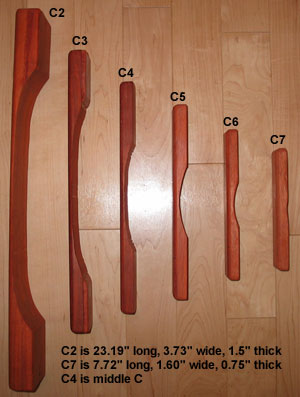
\includegraphics[height=200px]{marimba_bars.jpg}
		\caption{Vista lateral}
		\label{fig:marimba_bars_side}
	\end{subfigure}
	\hfill
	\begin{subfigure}{0.45\textwidth}
		\centering
		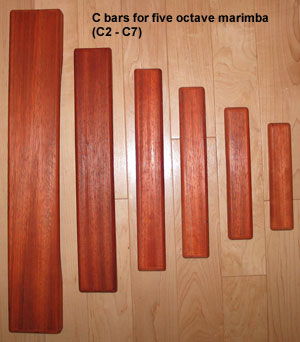
\includegraphics[height=200px]{marimba_bars-top.jpg}
		\caption{Vista superior}
		\label{fig:marimba_bars_top}
	\end{subfigure}
	\caption{Vista lateral e superior das barras da marimba~\cite{lafavre_tuning_marimba}}
	\label{fig:marimba_bars}
\end{figure}

O movimento vibratório das barras é tratado, de maneira simplificada, como unidimensional, ou seja, as vibrações ocorrem ao longo do comprimento da barra, e considerando principalmente os modos transversais. Além disso, é importante considerar a influência dos modos longitudinais (originam frequências muito agudas) e torcionais. A figura~\ref{fig:modos_vibratorios} mostra os primeiros modos vibratórios de uma marimba.

\begin{figure}[h!]
	\centering
	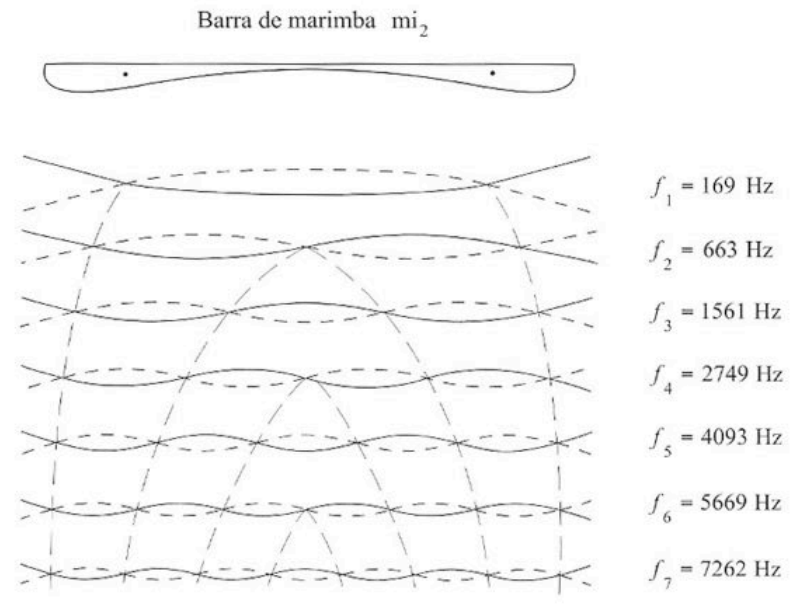
\includegraphics[width=0.6\textwidth]{modos_vibratorios.png}
	\caption{Esquema dos primeiros modos vibratórios de uma marimba (Rossing, 1976)~\cite{henrique2002acústica}}
	\label{fig:modos_vibratorios}
\end{figure}

As barras são suspensas por meio de uma corda de algodão com tensão regulável. A escolha do algodão é dada pela sua flexibilidade, o que evita que a corda não vibre por ressonância externa e introduza qualquer ruído indesejado. A importância da tensão ser regulável é destinada ao

\begin{itemize}
  \item Controle de vibração: uma corda muito tensa pode restringir a vibração das barras, enquanto uma muito frouxa pode não dar estabilidade o suficiente para as barras vibrarem adequadamente;
  \item Controle de altura das barras: a tensão adequada garante que uma sequência de barras, aos quais possuem tamanhos e massas variadas, estejam alinhadas.
\end{itemize}

As barras são percutidas por baquetas adequadas ao instrumento, sendo que as barras são excitadas em seu centro para maximizar a amplitude da vibração.

\subsection{Ressoadores}

Os ressoadores são tubos cilíndricos fechado-abertos posicionados abaixo de cada barra. Eles têm as funções de delinear a fundamental e amplificar a intensidade sonora. Em contrapartida, o tempo de decaimento do som é reduzido em comparação ao som da lâmina sem o dispositivo. Exemplificando com dados coletados por Fletcher e Rossing (1998), um som E5 a \SI{60}{\decibel} sem ressoador leva cerca de \SI{3.2}{\second} para decair, enquanto com ressoador, o tempo de decaimento é reduzido para \SI{1.5}{\second}.

Para formar uma onda estacionária com comprimento de onda $\lambda$, um tubo aberto-fechado deve ter o comprimento equivalente a $\lambda / 4$. Ou seja, o ressoador deve comportar $1/4$ do comprimento de onda da frequência fundamental da barra associada a ele. {Um detalhe importante é que apenas os modos ímpares são amplificados}\label{modos_impares}. A figura~\ref{fig:closed_open_pipe} mostra os três primeiros modos ímpares formados em um tubo fechado-aberto.

\begin{figure}[H]
	\centering
	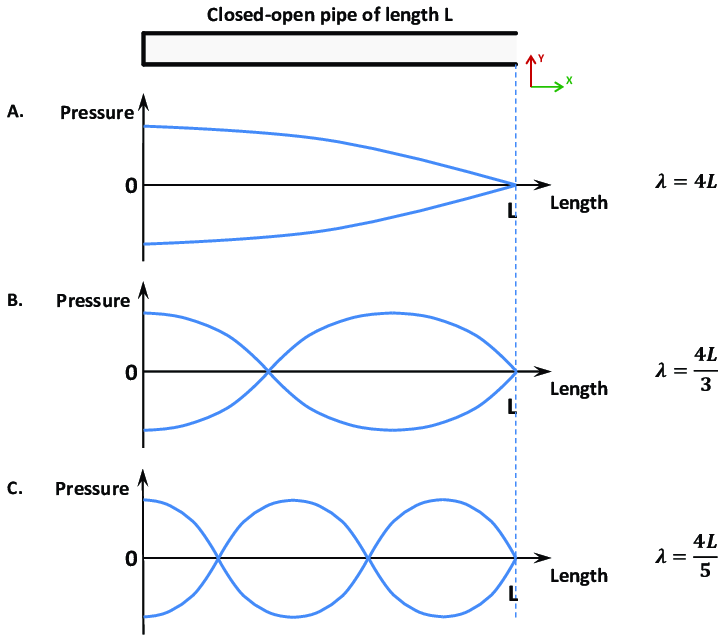
\includegraphics[width=0.6\textwidth]{Harmonics-of-a-closed-open-pipe-in-three-different-wavelengths-A-Four-times-the-length.png}
	\caption{Harmônicos de um tubo fechado-aberto em três comprimentos de onda diferentes: A. Quatro vezes o comprimento do tubo (4L) B. Quatro terços do comprimento do tubo (4L/3) e C. Quatro quintos do comprimento do tubo (4L/5)~\cite{closed_open_pipe}}
	\label{fig:closed_open_pipe}
\end{figure}

\section{Sonoridade}

A tessitura da marimba está contida no intervalo de A2 (\SI{110}{\hertz}) até C7 (\SI{2093}{\hertz}), sendo que os graves podem ser estendidos até C2 (\SI{65}{\hertz}).
As barras são afinadas para os modos 1, 4, 9 e 10. Entretanto, pela razão descrita em~\ref{modos_impares}, apenas os modos 1 e 9 são amplificados pelos ressoadores. Além disso, pelo uso de baquetas macias (ao menos em comparação com as baquetas do xilofone), a sonoridade resultante é carazterizada por ser cheia e escura.Jk

\bibliographystyle{plain}
\bibliography{references}

\end{document}